\documentclass[tikz,border=10pt,multi=tikzpicture]{standalone}
\usepackage{amsmath}
\usepackage{xcolor}

\definecolor{mainblue}{HTML}{001158}
\definecolor{accent}{HTML}{8592bc}
\definecolor{lightaccent}{HTML}{e7e9f2}

\begin{document}

% ===== German =====
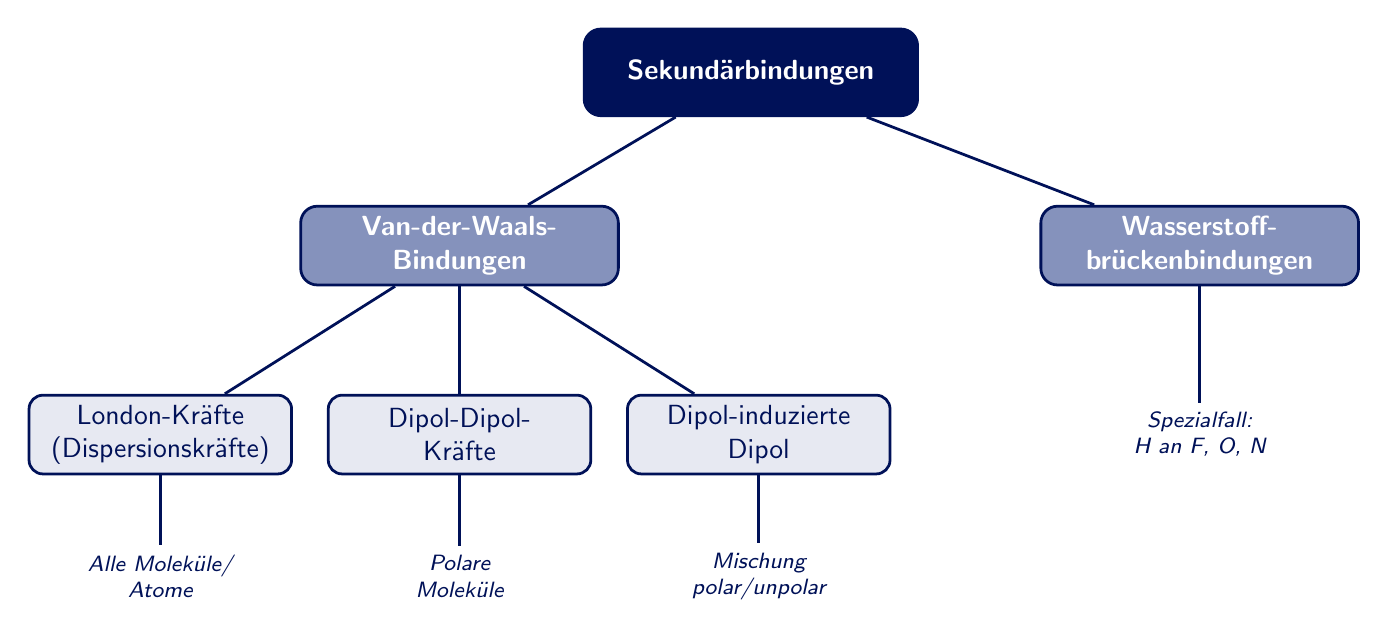
\begin{tikzpicture}[
    font=\sffamily,
    root/.style={
        rectangle, rounded corners=6pt, draw=mainblue, fill=mainblue, text=white,
        align=center, text width=4.0cm, minimum height=1.1cm, line width=1pt, font=\sffamily\bfseries
    },
    cat/.style={
        rectangle, rounded corners=6pt, draw=mainblue, fill=accent, text=white,
        align=center, text width=3.8cm, minimum height=1.0cm, line width=1pt, font=\sffamily\bfseries
    },
    leaf/.style={
        rectangle, rounded corners=5pt, draw=mainblue, fill=lightaccent, text=mainblue,
        align=center, text width=3.1cm, minimum height=1.0cm, line width=1pt, font=\sffamily
    },
    note/.style={
        align=center, text width=3.1cm, text=mainblue, font=\sffamily\itshape\footnotesize
    },
    edge/.style={draw=mainblue, line width=1pt}
]

\node[root] (root) at (-1.5,8.3) {Sekundärbindungen};

\node[cat] (vdw) at (-5.2,6.1) {Van-der-Waals-\\Bindungen};
\node[cat] (hbr) at (4.2,6.1)  {Wasserstoff-\\brückenbindungen};

\draw[edge] (root) -- (vdw);
\draw[edge] (root) -- (hbr);

\node[leaf] (lon) at (-9.0,3.7) {London-Kräfte\\(Dispersionskräfte)};
\node[leaf] (dd)  at (-5.2,3.7) {Dipol-Dipol-\\Kräfte};
\node[leaf] (did) at (-1.4,3.7) {Dipol-induzierte\\Dipol};

\draw[edge] (vdw) -- (lon);
\draw[edge] (vdw) -- (dd);
\draw[edge] (vdw) -- (did);

\node[note] (n1) at (-9.0,1.9) {Alle Moleküle/\\Atome};
\node[note] (n2) at (-5.2,1.9) {Polare\\Moleküle};
\node[note] (n3) at (-1.4,1.9) {Mischung\\polar/unpolar};
\node[note] (n4) at (4.2,3.7)  {Spezialfall:\\H an F, O, N};

\draw[edge] (lon) -- (n1);
\draw[edge] (dd)  -- (n2);
\draw[edge] (did) -- (n3);
\draw[edge] (hbr) -- (n4);

\end{tikzpicture}

% ===== English =====
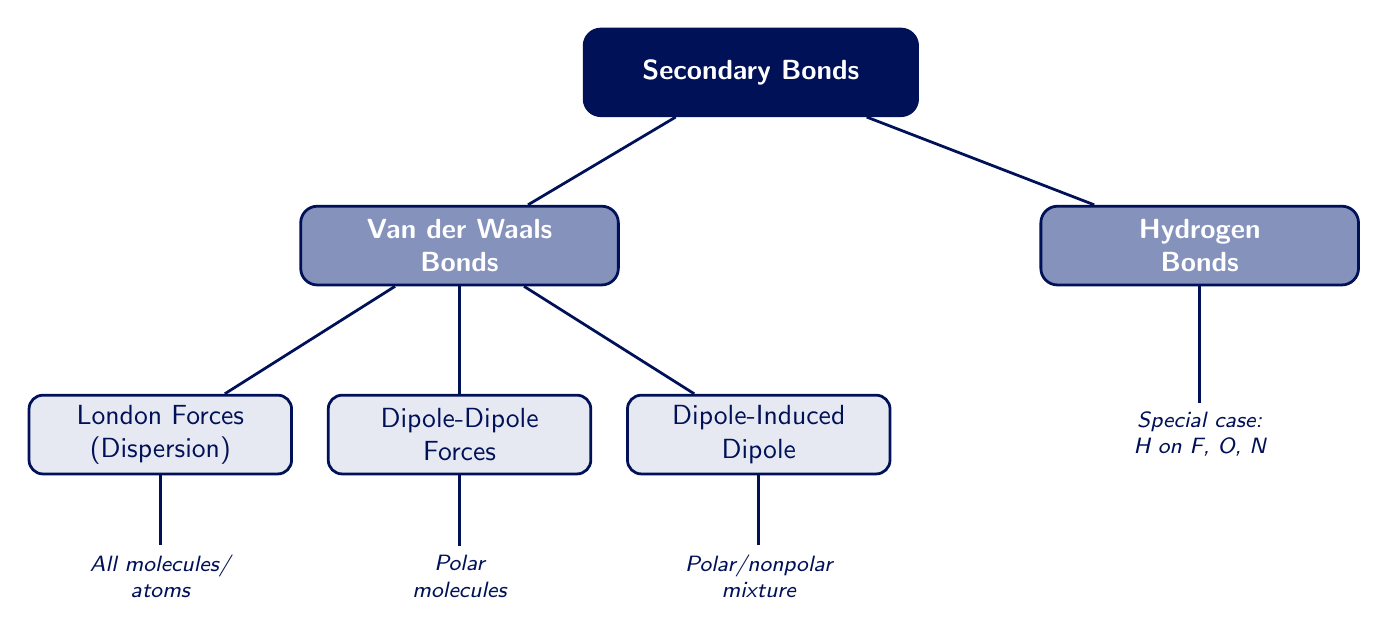
\begin{tikzpicture}[
    font=\sffamily,
    root/.style={
        rectangle, rounded corners=6pt, draw=mainblue, fill=mainblue, text=white,
        align=center, text width=4.0cm, minimum height=1.1cm, line width=1pt, font=\sffamily\bfseries
    },
    cat/.style={
        rectangle, rounded corners=6pt, draw=mainblue, fill=accent, text=white,
        align=center, text width=3.8cm, minimum height=1.0cm, line width=1pt, font=\sffamily\bfseries
    },
    leaf/.style={
        rectangle, rounded corners=5pt, draw=mainblue, fill=lightaccent, text=mainblue,
        align=center, text width=3.1cm, minimum height=1.0cm, line width=1pt, font=\sffamily
    },
    note/.style={
        align=center, text width=3.1cm, text=mainblue, font=\sffamily\itshape\footnotesize
    },
    edge/.style={draw=mainblue, line width=1pt}
]

\node[root] (root) at (-1.5,8.3) {Secondary Bonds};

\node[cat] (vdw) at (-5.2,6.1) {Van der Waals\\Bonds};
\node[cat] (hbr) at (4.2,6.1)  {Hydrogen\\Bonds};

\draw[edge] (root) -- (vdw);
\draw[edge] (root) -- (hbr);

\node[leaf] (lon) at (-9.0,3.7) {London Forces\\(Dispersion)};
\node[leaf] (dd)  at (-5.2,3.7) {Dipole-Dipole\\Forces};
\node[leaf] (did) at (-1.4,3.7) {Dipole-Induced\\Dipole};

\draw[edge] (vdw) -- (lon);
\draw[edge] (vdw) -- (dd);
\draw[edge] (vdw) -- (did);

\node[note] (n1) at (-9.0,1.9) {All molecules/\\atoms};
\node[note] (n2) at (-5.2,1.9) {Polar\\molecules};
\node[note] (n3) at (-1.4,1.9) {Polar/nonpolar\\mixture};
\node[note] (n4) at (4.2,3.7)  {Special case:\\H on F, O, N};

\draw[edge] (lon) -- (n1);
\draw[edge] (dd)  -- (n2);
\draw[edge] (did) -- (n3);
\draw[edge] (hbr) -- (n4);

\end{tikzpicture}

\end{document}
